\section{Introduction}


\begin{table*}[t]
    \footnotesize
    \centering
    \renewcommand{\arraystretch}{1.05}
    \setlength{\tabcolsep}{5.5pt}
    \caption{
        \textbf{Architectural details and main results of DEIMv2 variants.} We report the configurations for different variants and the final Average Precision (AP) on the COCO benchmark.
    }
    \vspace*{-2mm}
    \begin{tabular*}{\textwidth}{l | lcccccccc | ccc | c}
        \toprule
        \hline
        \multirow{2}{*}{\textbf{Variant}} & \multicolumn{2}{c}{\textbf{Backbone}} & \multicolumn{3}{c}{\textbf{Hidden Dimension}} & \multicolumn{2}{c}{\textbf{Layers}}  & \multirow{2}{*}{\textbf{\#Scales}} & \multirow{2}{*}{\textbf{\#Query}}  & \multirow{2}{*}{\textbf{\#Params}} & \multirow{2}{*}{\textbf{GFLOPs}} & \multirow{2}{*}{\textbf{Latency}} & \multirow{2}{*}{\textbf{AP}} \\
        & \textbf{Model} & \textbf{Adapter} & $\mathbf{d_{Back.}}$ & $\mathbf{d_{Enc.}}$ & $\mathbf{d_{Dec.}}$ & \textbf{\#$_{\text{Back.}}$} & \textbf{\#$_{\text{Dec.}}$} & & & & & & \\
        \midrule
        \hline
        X & ViT-S+ & STA & 384 & 256 & 256 & 12 & 6 & 3 & 300 & 50.26 & 151.6 & 13.75 & 57.8 \\
        L & ViT-S & STA & 384 & 256 & 256 & 12 & 4 & 3 & 300 & 32.18 & 96.32 & 10.47 & 56.0 \\
        M & ViT-T+ & STA & 256 & 256 & 256 & 12 & 4 & 3 & 300 & 18.11 & 52.20 & 8.80 & 53.0 \\
        S & ViT-T  & STA & 192 & 192 & 192 & 12 & 4 & 3 & 300 & 9.71 & 25.62 & 5.78 & 50.9 \\
        \midrule
        Nano & HGv2-B0 & - & 1024 & 128 & 128 & 5 & 3 & 2 & 300 & 3.57 & 6.86 & 2.32 & 43.0 \\
        Pico & HGv2-P & - & 512 & 112 & 112 & 4 & 3 & 2 & 200 & 1.51 & 5.15 & 2.14 & 38.5 \\
        Femto & HGv2-F & - & 256 & 96 & 96 & 3 & 3 & 2 & 150 & 0.96 & 1.67 & 1.91 & 31.0 \\
        Atto & HGv2-A & - & 256 & 64 & 64 & 3 & 3 & 2 & 100 & 0.49 & 0.76 & 1.61 & 23.8 \\
        \bottomrule
    \end{tabular*}
    \label{tab:main}
\end{table*}
Real-time object detection~\cite{redmon2016you,yolo11,tian2025yolov12,zhao2024detrs} is a critical component in many practical applications, including autonomous driving~\cite{liang2022edge}, robotics~\cite{maji2024yolo}, and industrial defect detection~\cite{hussain2023yolo}. Achieving a good balance between detection performance and computational efficiency remains a key challenge, especially for lightweight models suitable for edge and mobile devices. 

Among prevailing real-time detectors, DETR-based methods are increasingly favored for their end-to-end nature. Despite the robust feature representations offered by DINOv3~\cite{simeoni2025dinov3} in diverse scenarios, the feasibility and effectiveness of integrating it into DETR-based models have yet to be fully investigated.




In this work, we introduce DEIMv2, a real-time object detector built upon our previous DEIM~\cite{huang2025deim} pipeline and enhanced with DINOv3~\cite{simeoni2025dinov3} features. DEIMv2 employs official DINOv3-pretrained backbones (ViT-Small and ViT-Small+) for its largest variants (L and X sizes) to maximize feature richness, while its S and M variants leverage ViT-Tiny and ViT-Tiny+ backbones distilled from DINOv3, carefully balancing performance and efficiency. To address ultra-lightweight scenarios, we further introduce four specialized variants: Nano, Pico, Femto, and Atto, extending DEIMv2’s scalability across a wide spectrum of computational budgets.

To better leverage the strong feature representations of DINOv3, pretrained on large-scale data, under real-time constraints, we design the Spatial Tuning Adapter (STA). Operating in parallel with DINOv3, STA efficiently converts its single-scale outputs into the multi-scale features required for object detection in a parameter-free manner. Simultaneously, it performs fast downsampling of the input image to provide fine-grained, multi-scale detail features with very small receptive fields, complementing DINOv3’s strong semantics.

We further simplify the decoder by drawing on advances from the Transformer community. Specifically, we replace the conventional FFN and LayerNorm with SwishFFN~\cite{shazeer2020glu} and RMSNorm~\cite{zhang2019root}, both of which have been shown to be efficient without significantly affecting performance. We additionally note that object query locations change minimally during iterative refinement, motivating sharing query position embeddings across all decoder layers. Beyond this, we enhance Dense O2O by introducing object-level Copy-Blend augmentation, which increases effective supervision and further improves model performance.


\begin{figure*}[t]
    \centering
    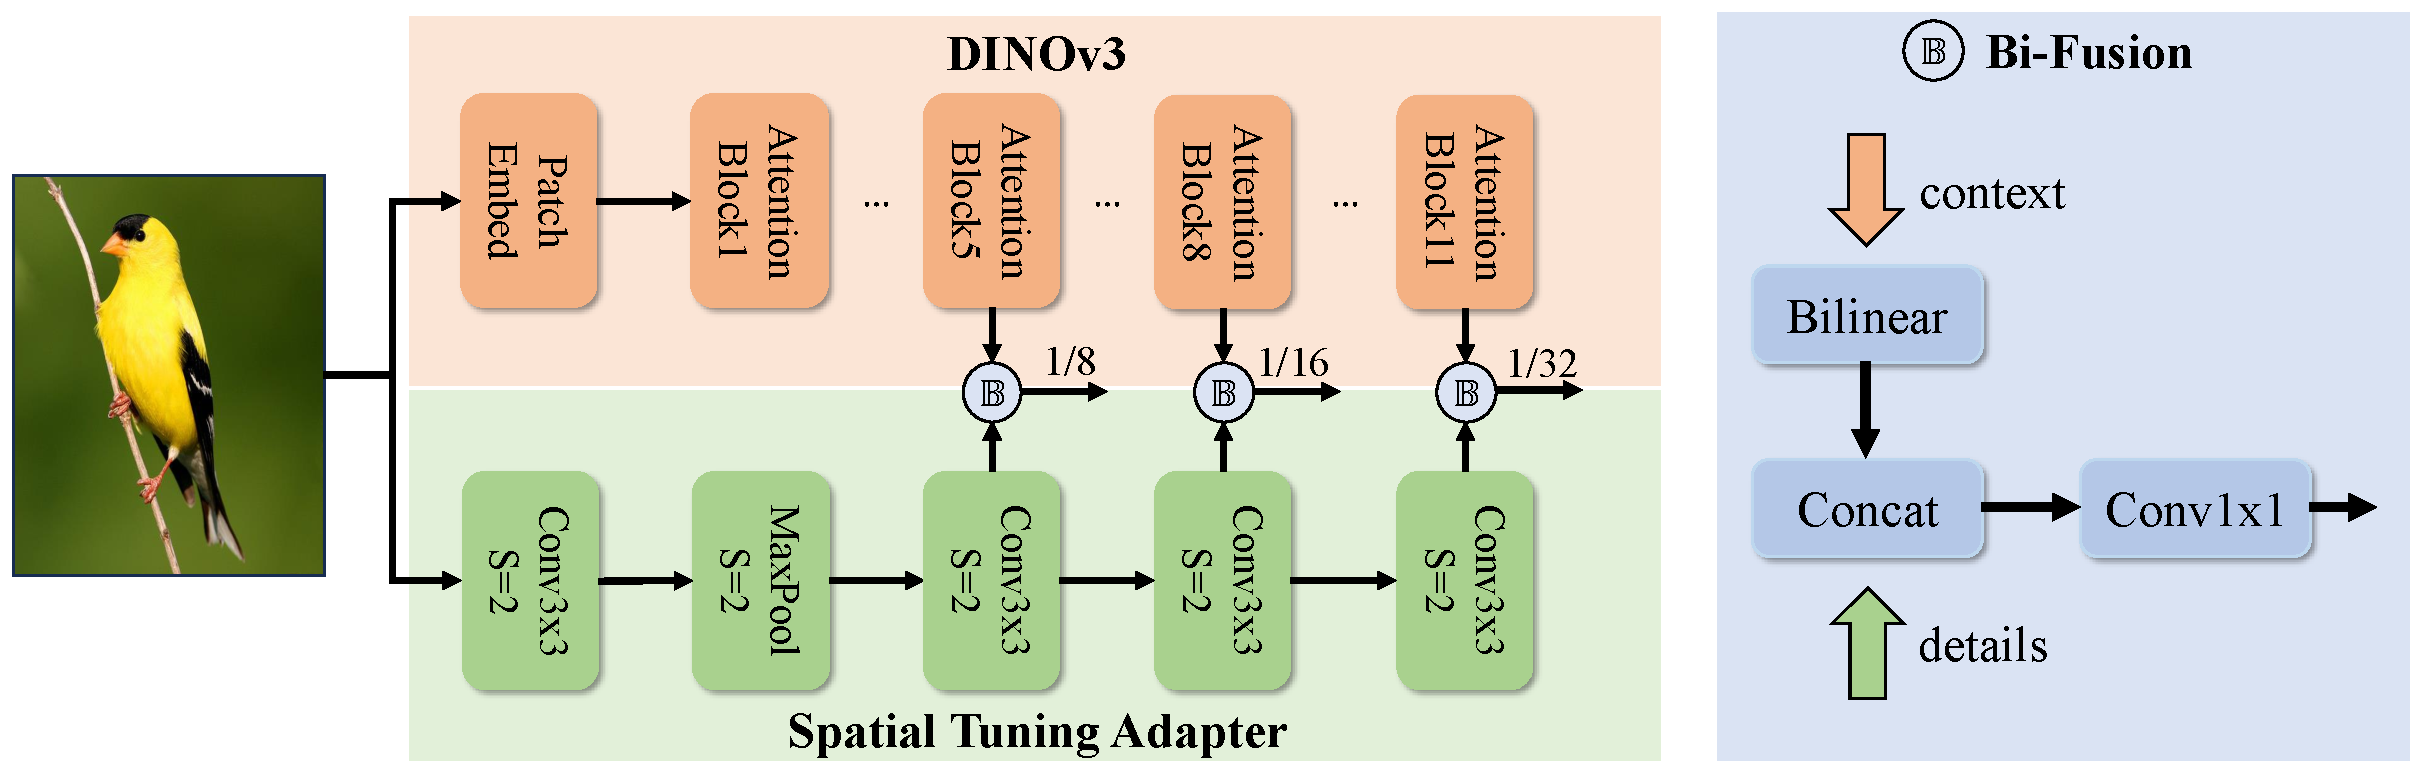
\includegraphics[width=\linewidth]{figures/STA_ver3.pdf}
    \caption{\textbf{Backbone design of our ViT-based variants}. We integrate DINOv3 with the proposed Spatial Tuning Adapter (STA).}
    \label{fig:STA}
\end{figure*}

Extensive experiments on COCO~\cite{lin2014microsoft} demonstrate that DEIMv2 achieves state-of-the-art performance across multiple model scales, which can be seen in Figure~\ref{fig:teaser}. Despite its simplicity, the family of DEIMv2 exhibits strong performance. For instance, our largest variant, DEIMv2-X, achieves 57.6 AP on COCO with only 50.3M parameters, surpassing prior best X-scale detectors DEIM-X that requires over 60M parameters yet attains only 56.5 AP. At the smaller end, DEIMv2-S establishes a notable milestone as the first model with fewer than 10M parameters to exceed 50 AP, highlighting the effectiveness of our design at compact scales. Furthermore, our ultra-lightweight DEIMv2-Pico, with merely 1.5M parameters, attains 38.5 AP, matching the performance of YOLOv10-Nano (2.3M parameters) while reducing parameter count by $\sim$50\%, thereby redefining the efficiency–accuracy frontier at the extreme lightweight regime. 

Our work highlights how DINOv3~\cite{simeoni2025dinov3} features can be effectively adapted for real-time object detection and provides a versatile framework spanning ultra-lightweight to high-performance models. To our knowledge, this is the first work in real-time object detection to simultaneously address such a wide range of deployment scenarios.

The main contributions of this work are summarized as follows:

\begin{itemize}

\item We present DEIMv2, which offers eight model sizes covering GPU, edge, and mobile deployment.

\item For larger models, we leverage DINOv3 for strong semantic features and introduce the STA to efficiently integrate them into real-time object detection.

\item For ultra-lightweight models, we leverage expert knowledge to effectively prune the depth and width of HGNetv2-B0, meeting strict computational constraints. 

\item Beyond backbone, we further simplify the decoder and upgrade Dense O2O, pushing the performance boundaries even further.

\item Finally, we demonstrate on COCO that DEIMv2 outperforms existing state-of-the-art methods across all resource settings, establishing new SOTA results.

\end{itemize}
